\documentclass[bachelor, och, labwork]{shiza}

\usepackage[utf8]{inputenc}
\usepackage{graphicx}

\usepackage[sort,compress]{cite}
\usepackage{amsmath}
\usepackage{amssymb}
\usepackage{amsthm}
\usepackage{fancyvrb}
\usepackage{longtable}
\usepackage{array}
\usepackage[english,russian]{babel}
\usepackage{minted}

\usepackage{tempora}


% \usepackage[colorlinks=false]{hyperref}


\newcommand{\eqdef}{\stackrel {\rm def}{=}}


\begin{document}

\title{Алгоритмы алгебры и теории чисел}

\course{4}

\group{431}

\napravlenie{10.05.01 "--- Компьютерная безопасность}


\author{Никитина Арсения Владимировича}


\satitle{доцент}
\saname{А.\,С.\,Гераськин}


\date{2022}

\maketitle

% Включение нумерации рисунков, формул и таблиц по разделам
% (по умолчанию - нумерация сквозная)
% (допускается оба вида нумерации)
%\secNumbering


\tableofcontents

\section{Задание лабораторной работы}

Реализация алгоритма полиномиального деления (PDF).

\section{Теоретическая часть}

\begin{center}
    \textit{Полиномиальное деление над полем (Polynomial Division
    over a Field)}
\end{center}

\textit{Вход:} $p_1(x) = \sum^{m}_0 c_ix^i$ и $p_2(x) = \sum^{n}_0 c_ix^i$ над
полем $f$, $n\in\overline{0,m}$ и $d_n \not=0$. (Этот алгоритм будет работать и 
над областью целостности $J$ при условии, что $d_n$ обратим в $J$.)

\textit{Выход:} $q(x) = \sum^{m-n}_{0} q_ix^i$ и $r(x) = \sum^{n-1}_{0} r_ix^i$,
обладающие свойством евклидовости.

\begin{enumerate}
    \item Для $k$ от $m-n$ до $0$ выполнять:
    \begin{enumerate}
        \item $q_k= c_{n+k}/d_n$.
        \item Для $j$ от $n + k - 1$ до $0$ выполнять:
        \begin{enumerate}
            \item $c_j=c_j-q_kd_{j-k}.$
        \end{enumerate}
    \end{enumerate}
    \item Ответ --- $q_i, ~i=\overline{0, m - n}$, коэффициенты полинома $q(x)$,
    вычисленного на шаге 1, и $r_i, ~i=\overline{0, n - 1}$, коэффициенты
    полинома $r(x)$, где $r_i=c_i$.

\end{enumerate}


\section{Практическая часть}
\subsection{Пример работы алгоритма}
\begin{figure}[H]
    \centering
    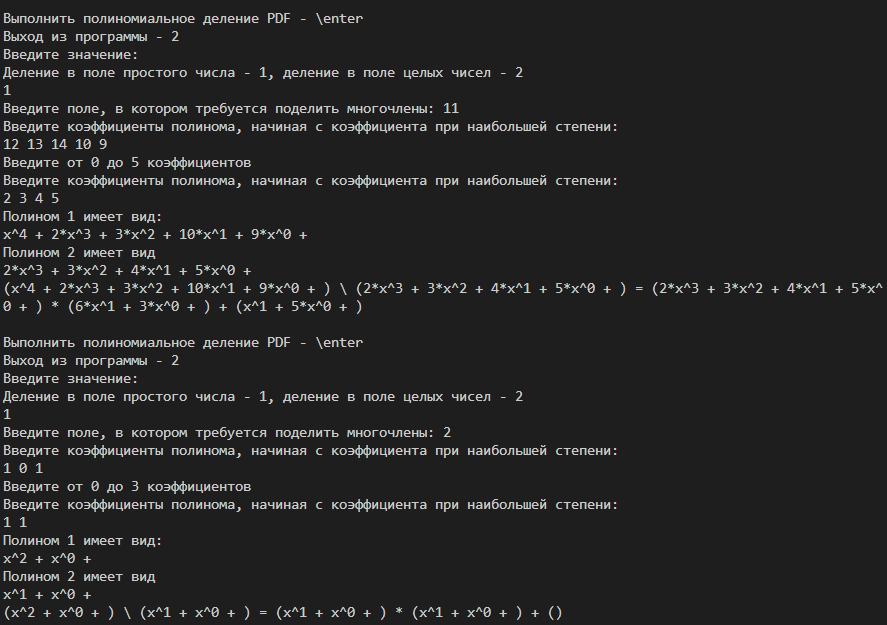
\includegraphics[width=1\textwidth]{pic1.png}
    \caption{}
\end{figure}

\setminted[python]{linenos,breaklines=true, fontsize=\small, style=bw}
    \subsection{Код программы, реализующей рассмотренный алгоритм}
        \inputminted{python}{lab13.py}


\end{document}